\documentclass[12pt,a4paper]{article}

\usepackage[utf8]{inputenc}
\usepackage[T1]{fontenc}
\usepackage{geometry}
\geometry{margin=1in}
\usepackage{graphicx}
\usepackage{xcolor}
\usepackage{titlesec}
\usepackage{hyperref}
\usepackage{tcolorbox}
\usepackage{float}
\usepackage{enumitem}
\usepackage{listings}
\usepackage{tikz}

% Custom Colors
\definecolor{EUIBlue}{HTML}{1A73E8}
\definecolor{DarkNavy}{HTML}{0B192E}
\definecolor{CodeBg}{HTML}{F1F5F9}

% Code Style
\lstset{
    backgroundcolor=\color{CodeBg},
    basicstyle=\ttfamily\small,
    breaklines=true,
    frame=single,
    rulecolor=\color{lightgray},
    keywordstyle=\color{EUIBlue}\bfseries,
    stringstyle=\color{green!60!black},
    commentstyle=\color{gray}
}

% Links setup
\hypersetup{
    colorlinks=true,
    linkcolor=EUIBlue,
    filecolor=magenta,      
    urlcolor=EUIBlue,
}

\begin{document}

% ==========================================
% TITLE PAGE
% ==========================================
\begin{titlepage}
    \centering
    \vspace*{4cm}
    {\Huge \textbf{EUI OMR ENGINE}} \\[0.5cm]
    {\LARGE Technical Documentation \& User Guide} \\[2cm]
    
    {\large \textbf{Version:}} 1.1.1 \\
    {\large \textbf{Author:}} Mustafa Mahmoud \\[2cm]
    
    \vfill
    {\large \today}
\end{titlepage}

\newpage
\tableofcontents
\newpage

% ==========================================
% ABSTRACT
% ==========================================
\begin{abstract}
Educational grading at scale demands precision, speed, and reliability. The EUI Optical Mark Recognition (OMR) Engine resolves the persistent cost and inflexibility of legacy hardware scanners by providing a 100\% software-based, computer vision solution. This document comprehensively outlines the architecture, setup, algorithms, and operational usage of the EUI OMR Engine.
\end{abstract}

% ==========================================
% INTRODUCTION
% ==========================================
\section{Introduction}

\subsection{The Problem}
Standardized testing traditionally relies on specialized hardware OMR scanners and proprietary paper. This paradigm is rigid, prohibitively expensive to maintain, and brittle to human error. A faint pencil stroke, a stray smudge, or a skewed paper feed frequently aborts autonomous grading, forcing faculty into tedious manual remarking processes.

\subsection{Target Users}
\begin{itemize}
    \item \textbf{University Administrators \& Operational Staff}: To rapidly grade batches of tests and safely export data to student information systems.
    \item \textbf{Professors \& Teaching Assistants}: To customize exam answer keys and resolve ambiguous student entries visually.
    \item \textbf{Developers}: To maintain, extend, and adapt the underlying image processing pipelines or configuration bounds.
\end{itemize}

% ==========================================
% SYSTEM OVERVIEW
% ==========================================
\section{System Overview}

\subsection{High-Level Architecture}
The system is constructed with a modular, decoupled architecture prioritizing data integrity and asynchronous processing. 
\begin{itemize}
    \item \textbf{Presentation Layer (UI)}: Built with PySide6 (Qt framework) enforcing thread-isolated UI updates and a dark-theme, glassmorphism design language.
    \item \textbf{Computer Vision Core}: Python-based image processing utilizing OpenCV (\texttt{cv2}) for geometrical transformations and NumPy for high-speed matrix density calculations.
    \item \textbf{Data Ingestion Layer}: Employs PyMuPDF (\texttt{fitz}) for vector-to-raster PDF extraction and \texttt{openpyxl/pandas} for bidirectional Excel dataset bridging.
\end{itemize}

\subsection{Workflow Diagram}
\begin{figure}[H]
    \centering
    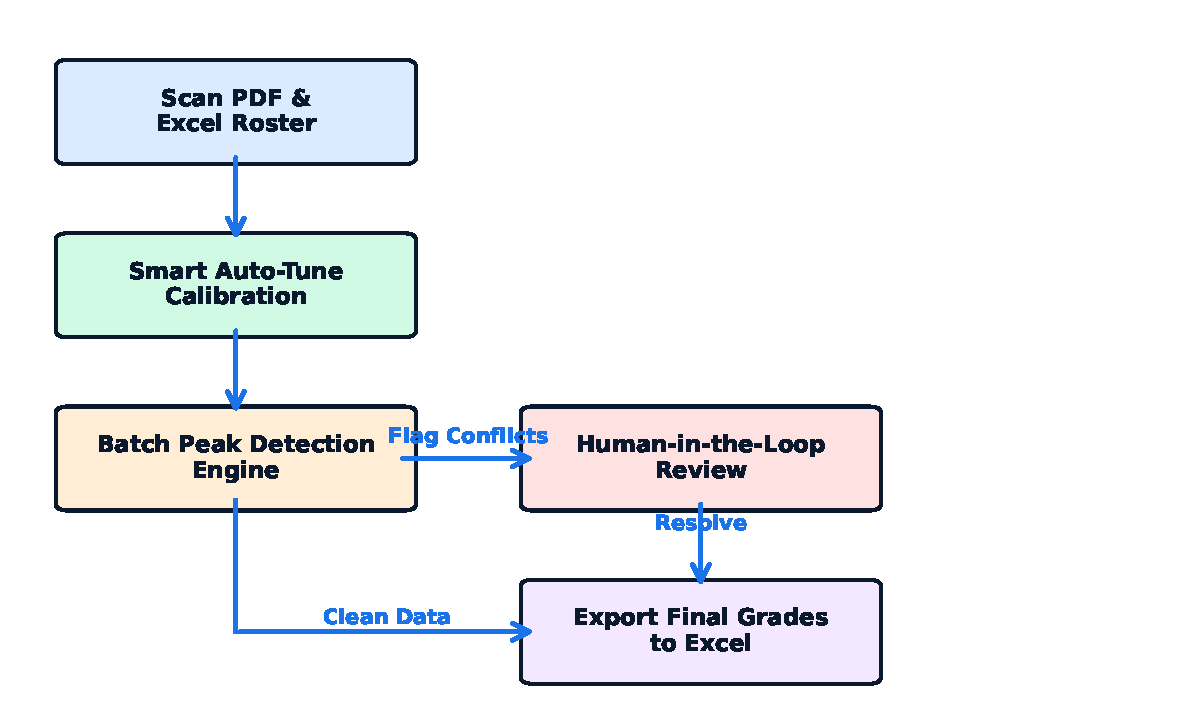
\includegraphics[width=\linewidth]{workflow_diagram.pdf}
    \caption{Process Data Flow}
\end{figure}

% ==========================================
% INSTALLATION GUIDE
% ==========================================
\section{Installation Guide}

\subsection{Production Deployment (Recommended)}
The EUI OMR Engine is distributed as a portable, standalone executable folder for Windows platforms.
\begin{enumerate}
    \item Download the latest release (\texttt{EUI\_OMR\_Engine\_v1.1.1\_Win.zip}).
    \item Extract the ZIP folder to your desktop or desired secure drive.
    \item Run \texttt{EUI\_OMR\_Engine.exe}. No local Python installation or administrative privileges are required.
\end{enumerate}

\subsection{Development Environment Setup}
\begin{lstlisting}[language=bash]
# Clone repository
git clone https://github.com/MustafaMahmoud-ILE/eui_omr.git
cd eui_omr

# Setup Virtual Environment
python -m venv .venv
source .venv/Scripts/activate

# Install Dependencies
pip install -r requirements.txt

# Run Application
python main_entry.py
\end{lstlisting}

% ==========================================
% USAGE GUIDE
% ==========================================
\section{Usage Guide}

\subsection{Basic Workflow}
\begin{enumerate}
    \item \textbf{Setup Phase}: Select the destination Excel roster, map the ID/Grade columns, and upload the batch PDF of student scans.
    \item \textbf{Key Configuration}: Select the correct models (A, B, C, D) for the exam questions via manual UI selection or model scanning.
    \item \textbf{Initiate Grading}: Click \textbf{Start}. The engine silently tunes its sensitivity, processes the batch, and renders the Results Dashboard.
    \item \textbf{Review \& Export}: Correct any red error rows via double-clicking, then export back to Excel.
\end{enumerate}

% ==========================================
% FEATURES
% ==========================================
\section{Features}

\subsection{Smart Calibration (Auto-Tuning)}
Desk scanners lack optical consistency. The engine counters this by extracting 5 random, valid pages and systematically stepping through binary threshold coefficients. It identifies the exact density matrix value that distinguishes graphite from paper for the current specific hardware run.

\subsection{Probabilistic Peak Detection}
The engine measures relative darkness within an array (e.g., all 10 bubbles of an ID column). It identifies the statistical "Peak" of darkness. This allows successful reads of faint marks while ignoring poor erasures or stray pencil noise.

\subsection{Human-in-the-Loop Conflict Resolution}
No automated system is flawless. When mathematical ambiguity occurs, grading halts for that specific test, and the visual crop is relayed to a GUI modal for operator override.

% ==========================================
% ARCHITECTURE DETAILS
% ==========================================
\section{Architecture Details}

\subsection{Image Perspective Transformation}
The core OMR function, \texttt{process\_array()}, utilizes a 4-point perspective transform. The scanner often feeds paper slightly skewed. The engine hunts for 4 defined geometric corner markers in the image space. Using \texttt{cv2.getPerspectiveTransform()}, it aligns the skewed space into a perfectly orthogonal layout. Coordinate \texttt{(X, Y)} is then guaranteed to house the correct bubble.

\subsection{Data Models \& Concurrency}
Internal state is passed between threads using immutable Data Classes (e.g., \texttt{GradingResult}, \texttt{ProjectManager}). The heavy image processing logic is strictly detached into QThread worker classes (e.g., \texttt{PDFGraderWorker}, \texttt{AutoTuneWorker}) employing Signal/Slot emission to update the UI safely without blocking the main event loop.

% ==========================================
% CONFIGURATION
% ==========================================
\section{Configuration}

\subsection{\texttt{config.json}}
The Region of Interest (ROI) definitions are exclusively isolated from Python code in an editable \texttt{config.json} located parallel to the runtime executable. This allows administrative adjustment of bounding boxes when the physical exam paper template is altered.

\begin{lstlisting}
{
  "student_id": { "x": 1081, "y": 801, "w": 381, "h": 286 },
  "version": { "x": 1081, "y": 1289, "w": 381, "h": 129 },
  "corners": { "tl_x": 84, "tl_y": 74 }
}
\end{lstlisting}

% ==========================================
% SECURITY CONSIDERATIONS
% ==========================================
\section{Security Considerations}

\subsection{Architecture Overview}
The EUI OMR Engine processes sensitive educational data falling strictly within local administrative policies. 
\begin{itemize}
    \item \textbf{Offline Architecture}: The engine operates 100\% client-side. No telemetry, student responses, or grades ever traverse a network or API boundary.
    \item \textbf{Auditability}: Manual overrides are explicitly tracked and logged in the raw data structures, establishing a verification trail if an appeal is filed by a student.
\end{itemize}

% ==========================================
% TROUBLESHOOTING
% ==========================================
\section{Troubleshooting}

\begin{itemize}
    \item \textbf{Error: Multiple Pages Skipped}: Ensure the PDF was scanned right-side up or upside down. If the document is fed in \textit{Landscape}, the corner markers will fail to register.
    \item \textbf{Error: Cannot Export to Excel}: Close the target \texttt{.xlsx} file in Microsoft Excel. Excel places write-locks on open files, preventing the engine from injecting grades.
    \item \textbf{Error: "Config Not Found" fallback warning}: Ensure \texttt{config.json} sits directly adjacent to \texttt{EUI\_OMR\_Engine.exe}.
\end{itemize}

% ==========================================
% FUTURE IMPROVEMENTS
% ==========================================
\section{Future Improvements}
\begin{itemize}
    \item \textbf{Multi-Processing Processing Pipeline}: While UI concurrency is solved, the grading logic remains CPU-bound on a single core. Implementing \texttt{multiprocessing} could chunk PDF loads across all CPU threading pools, significantly accelerating 1,000+ page batches.
    \item \textbf{Visual ROI Configurator}: A graphical tool enabling standard users to draw boxes over a PDF to generate the \texttt{config.json} arrays visually rather than typing integer coordinates.
    \item \textbf{Barcode Integration}: Scanning QR or Barcodes for automatic versioning control rather than relying on bubble input.
\end{itemize}

% ==========================================
% APPENDIX
% ==========================================
\section{Appendix}
For further questions or contributions, access the source repository: \\
\url{https://github.com/MustafaMahmoud-ILE/eui_omr}

\end{document}
